\chapter{Tính toán chuỗi Markov}
%%%%%%%%%%%% Anh Tu%%%%%%%%%%%%%%%%
% \section{định nghĩa ma trận markov:}

% \begin{defivn}
%     \textbf{Ma trận Markov}, hay còn được gọi là \textbf{ma trận ngẫu nhiên} được dùng để miêu tả các trạng thái trong chuỗi Markov. Ma trận Markov có các đặc trưng sau:
%     \begin{itemize}
%         \item 
%     \end{itemize}
% \end{defivn}
% \begin{itemize}
%     \item 
% \end{itemize}
%%%%%%%%%%%%%Le Ngu%%%%%%%%%%%%%%%%
\section{Luỹ thừa ma trận}

\begin{itemize}
    \item Xét một chuỗi Markov có $S = \{x_1, x_2, ..., x_n\}$ và một phân phối ban đầu $\pi_0$. 

    \item Để tính toán được $\pi_1$, áp dụng công thức xác suất đầy đủ, ta có:
    $$
    \begin{aligned}
    \pi_1(x_i) &= \P(X_1 = x_i) \\ 
    &= \sum_{j = 0}^{n} \P(X_0 = x_j)\P(X_1  = x_i \mid X_0 = x_j) \\
    &= \sum_{j = 0}^{n} \pi_0(x_j) P_{x_jx_i}
    \end{aligned}
    $$

    \item Ta có thể thấy $\pi_1(x_i)$ chính là tích vô hướng giữa vector dòng $\pi_0$ và cột thứ $i$ của ma trận $\mathbf{P}$. Vậy ta có:
    $$
    \pi_1 = \begin{bmatrix}
        \pi_1(x_1) & \pi_1(x_2) & \dotsb & \pi_1(x_n) \\
    \end{bmatrix} = \pi_0 \mathbf{P}
    $$

    \item Tiếp theo để tính được $\pi_2(x_i)$ ta tiếp tục áp dụng công thức xác suất đầy đủ:
    $$
    \begin{aligned}
    \pi_2(x_i) &= \P(X_2 = x_i) \\
    &= \sum_{j=0}^{n} \P(X_1 = x_j) \P(X_2 = x_i \mid X_1 = x_j) \\
    &= \sum_{j=0}^{n} \pi_1(x_j) \P(X_1 = x_i \mid X_0 = x_j) \\
    &= \sum_{j=0}^{n} \pi_1(x_j) P_{x_jx_i} \\
    &= \sum_{j=0}^{n} \left( \sum_{k=0}^{n} \pi_0(x_k) P_{x_kx_j} \right) P_{x_jx_i} \\
    &= \sum_{k=0}^{n} \pi_0(x_k) \left( \sum_{j = 0}^n P_{x_kx_j} P_{x_jx_i} \right)
    \end{aligned}
    $$

    \item Ta có thể thấy $\pi_2(x_j)$ chính là tích vô hướng giữa vector dòng $\pi_0$ và cột thứ $i$ của ma trận $\mathbf{P}^2$. Vậy ta có:
    $$
    \pi_2 = \begin{bmatrix}
        \pi_2(x_1) & \pi_2(x_2) & ... & \pi_2(x_n) \\
    \end{bmatrix} = \pi_0 \mathbf{P}^2
    $$

    \item Ta gọi $\P(X_2 = y \mid X_0 = x)$ là \textit{xác suất chuyển tiếp 2-bước}. Tương tự với $\P(X_n = y \mid X_0 = x)$ ta gọi là \textit{xác suất chuyển tiếp n-bước}.

    \item Dựa vào xác suất chuyển tiếp 2-bước và 1-bước, ta có thể doán được:
    \begin{equation}
    \pi_n = \pi_0 \mathbf{P}^{n}
    \end{equation}
    
    \begin{proofvn} Ta sẽ dùng quy nạp để chứng minh. Đầu tiên ta đã chứng minh được phương trình (2.1) đúng với $n = 1$ và $n = 2$, giả sử $n = k$ đúng, nghĩa là:
    $$
    \pi_k = \pi_0 \mathbf{P}^k
    $$
    \noindent Xét $n = k+1$, ta có:
    $$ 
    \begin{aligned}
    \pi_{k+1}(x_i) &= \P(X_{k+1} = x_i) \\
    &= \sum_{j=0}^{n} \P(X_{k} = x_j) \P(X_{k+1} = x_i \mid X_k = x_j) \\
    &= \sum_{j=0}^{n} \P(X_{k} = x_j) \P(X_1 = x_i \mid X_0 = x_j) \\
    &= \sum_{j=0}^{n} \pi_{k}(x_j) P_{x_jx_i} \\
    \end{aligned}
    $$

    \noindent Ta có thể thấy $\pi_{k+1}(x_i)$ là tích vô hướng giữa vector dòng $\pi_k$ và cột thứ $i$ của ma trận chuyển tiếp $\mathbf{P}$, do đó:
    $$
    \pi_{k+1} = \pi_k \mathbf{P} = \pi_0 \mathbf{P}^{k} \mathbf{P} = \pi_0 \mathbf{P}^{k+1}
    $$

    \noindent Vậy theo quy nạp, phương trình (2.1) đúng với mọi $n \geq 1$.
    \end{proofvn}
\end{itemize}

\begin{defivn}
    Cho $(X_n)_{n \geq 0}$ là một chuỗi Markov với ma trận chuyển tiếp $\mathbf{P}$. Với mọi $n \geq 1$, ta gọi ma trận $\mathbf{P}^n$ là \textbf{ma trận chuyển tiếp n-bước}. Các phần tử của ma trận $\mathbf{P}^n$ được gọi là \textbf{xác suất chuyển tiếp n-bước}. Với mọi $x, y \in S$  ta kí hiệu xác suất chuyển tiếp n bước từ $x$ tới $y$ là $P^n_{xy}$.
\end{defivn}

\begin{itemize}
    \item Để dễ dàng hơn trong việc tính toán ma trận $\mathbf{P}^n$ ta có thể dùng phương pháp chéo hoá.
    \item Dùng tính chất của luỹ thừa, ta có:
    $$
    \pi_{n + m} = \pi_0 \mathbf{P}^{n + m} = \pi_0 \mathbf{P}^n \mathbf{P}^m
    $$

    \item Ngoài ra ta có:
    $$
    \P(X_n = y \mid X_0 = x) = P^n_{xy} \implies \P(X_{m + n} = y \mid X_{m} = x) = P^n_{xy}
    $$
\end{itemize}

%%%%%%%%%%%Nguyên Phương & vmthu%%%%%%%%%%%
\section{Trị riêng của ma trận markov}

% \begin{itemize}
% \end{itemize}

Các trị riêng của ma trận Markov có một số tính chất đặc biệt, các tính chất này giúp chúng ta có thể giải thích các tính chất của chuỗi Markov bằng ngôn ngữ của đại số tuyến tính một cách trực quan và dễ dàng hơn.

\begin{theovn}
Ma trận markov luôn có ít nhất một trị riêng bằng 1.
\end{theovn}
\begin{proofvn} \vphantom{text}
\begin{itemize}
    \item Với ma trận Markov $\mathbf{P}$ có kích thước $n \times n$, xét phương trình:
    \begin{align}
        \mathbf{P}\textbf{x} &= \textbf{x} \\
        (\mathbf{P} - I)\textbf{x} &= 0.
    \end{align}
   
    % \item Với $p_{ij}$ là phần tử hàng $i$ cột $j$ của $P$, $b_{ij}$ là phẩn tử hàng $i$ cột $j$ của $P - I$, $k \leq n$, ta có:
    \item Với $b_{ij}$ là phẩn tử hàng $i$ cột $j$ của $\mathbf{P} - I$, $k \leq n$, ta có:
    \begin{align}
        \sum_{j = 1}^{n}b_{kj} =  \sum_{j = 1}^{n}P_{kj} - 1 = 1 - 1 = 0.
    \end{align}

    \item Suy ra, với $\textbf{u}_i$ là các vector cột của $(\mathbf{P}-\lambda I)$, ta có:
    \begin{align}
        \sum_{i=1}^{n} \textbf{u}_i = 0.
    \end{align}

    \item Suy ra các các vector cột của $(\mathbf{P}-\lambda I)$ phụ thuộc tuyến tính, từ đó suy ra $r(\mathbf{P}) < n$, hay phương trình (2.2) luôn có nghiệm. 

    \item Vậy, vì $\lambda = 1$ thoả $\mathbf{P}$\textbf{x} = 1\textbf{x} nên 1 là trị riêng của $\mathbf{P}$.
\end{itemize}
\end{proofvn}

\begin{theovn}
Các trị riêng của ma trận Markov luôn bé hơn hoặc bằng 1.
\end{theovn}
\begin{proofvn}
    Chúng ta có thể chứng minh như sau:

    \begin{itemize}
        \item  Với ma trận Markov $\mathbf{P}$ có kích thước $n \times n$, $\lambda$ là 1 trị riêng của $\mathbf{P}$, ta có: 
        \begin{align}
            \mathbf{P}\textbf{x} = \lambda \textbf{x}
        \end{align}
    
        \item Xét hàng thứ $k$ của cả 2 vế, ta có:
        \begin{align}
            \sum_{j = 1}^n P_{kj}x_j = \lambda x_k
        \end{align}
    
        \item Đặt phần tử $x_m$ thoả:
        \begin{align}
            |x_m| = \max (|x_1|, |x_2|, ... ,|x_n|)
        \end{align}

        \item Lúc này, ta có:
        \begin{align}
            |\lambda x_m| = \left|\sum_{j = 1}^n P_{mj}x_j\right|
            \leq \sum_{j = 1}^n |P_{mj}x_j|           
            \leq \sum_{j = 1}^n |P_{mj}x_m|           
            = |x_m|\sum_{j = 1}^n |P_{mj}|         
            = |x_m|.1
        \end{align}
        
        \item Suy ra $\lambda \leq 1$
    \end{itemize}
\end{proofvn}
%%%% Le Ngu %%%%%%
\section{Ví dụ tiêu biểu}

\begin{probvn}
    Theo khảo sát của sinh viên đối với ba quán cafe $A, B, C$, ta biết rằng ban đầu, hai quán $A, B$ chưa mở nên $100\%$ khách đều đến $C$ và:
    \begin{itemize}
        \item Trong những sinh viên đến quán $A$, sẽ có $20\%$ người tiếp tục đến $A$, có $60\%$ người sang $B$ và có $20\%$ người sang $C$.
        \item Trong những sinh viên đến quán $B$, sẽ có $40\%$ người tiếp tục đến $B$, có $10\%$ người sang $A$ và có $50\%$ người sang $C$.
        \item Trong những sinh viên đến quán $C$, sẽ có $10\%$ người tiếp tục đến $C$, có $70\%$ người sang $A$ và có $20\%$ người sang $B$.
    \end{itemize}

    \begin{itemize}
        \item[(a)] Hãy tìm xem tỉ lệ phần trăm người đến quán $A$, $B$, $C$ sau 3 tuần.
        \item[(b)] Hãy tìm xem tỉ lệ sinh viên đến quán $B$ ở tuần thứ 5 biết rằng tuần thứ 2 ở quán $C$ và tuần thứ 3 ở quán $A$.
        \item[(c)] Hãy tìm xem tỉ lệ sinh viên đến quán $B$ ở tuần thứ 2 và đến quán $A$ ở tuần thứ 4 biết rằng đến quán $B$ ở tuần thứ 3.
    \end{itemize}
\end{probvn}

\noindent \textbf{Giải:} Thời gian chúng ta xét sẽ là tuần. Tiếp theo ta có không gian trạng thái $S = \{A, B, C \}$. Đặt $X_t$ là biến ngẫu nhiên đại diện cho quán cafe mà sinh viên đến ở tuần thứ $t$ và có phân phối ban đầu $\pi_0$ là
$$
\pi_0 = \begin{bmatrix}
\P(X_0 = A) & \P(X_0 = B) & \P(X_0 = C) 
\end{bmatrix} = \begin{bmatrix}
    0 & 0 & 1
\end{bmatrix}
$$

\noindent Dựa theo đề bài ta có ma trận chuyển tiếp $\mathbf{P}$ là:
$$
\mathbf{P} = \begin{bmatrix}
    P_{AA} & P_{AB} & P_{AC} \\
    P_{BA} & P_{BB} & P_{BC} \\
    P_{CA} & P_{CB} & P_{CC}
\end{bmatrix} = \begin{bmatrix}
    0.2 & 0.6 & 0.2 \\
    0.1 & 0.4 & 0.5 \\
    0.7 & 0.2 & 0.1
\end{bmatrix}
$$

\noindent Ta biểu diễn chuỗi Markov trên thành đồ thị như dưới đây:
\begin{figure}[H]
    \centering
    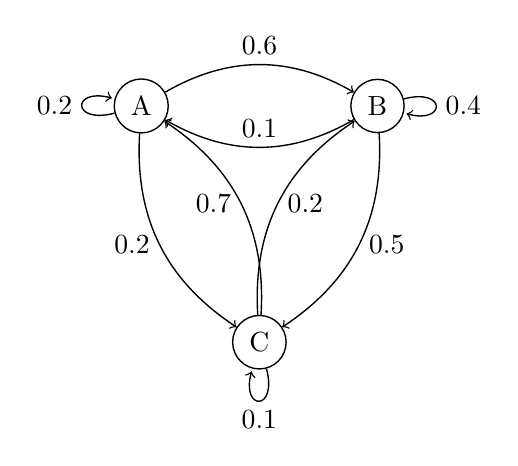
\begin{tikzpicture}[-> , line width=0.5 pt ,node distance =2 cm]
        %    \tikzstyle{every node}=[font=\large]
        
        \node[circle, draw] (A) at (0,0) {A};
        \node[circle, draw] (B) at (3,0) {B};
        \node[circle, draw] (C) at (1.5, -3) {C};
        
        \path (A) edge [bend left] node [above] {$0.6$} (B);
        \path (A) edge [loop left] node{$0.2$} (A);
        \path (A) edge [bend right] node [left] {$0.2$} (C);

        \path (B) edge [bend left] node [above] {$0.1$} (A);
        \path (B) edge [loop right] node{$0.4$} (B);
        \path (B) edge [bend left] node [right] {$0.5$} (C);

        \path (C) edge [bend right] node [left] {$0.7$} (A);
        \path (C) edge [bend left] node [right] {$0.2$} (B);
        \path (C) edge [loop below] node{$0.1$} (C);
        
    \end{tikzpicture}
    \caption{Đồ thị $G$ biểu diễn của chuỗi Markov của bài toán} 
    \label{fig:graphprob}
\end{figure}

\noindent Tính toán luỹ thừa 2 và 3 của ma trận chuyển tiếp $\mathbf{P}$, ta được:
$$
\mathbf{P}^2 = \begin{bmatrix}
    0.24 & 0.4 & 0.36 \\
    0.41 & 0.32 & 0.27 \\
    0.23 & 0.52 & 0.25
\end{bmatrix} \hspace{10pt} \text{và} \hspace{10pt}
\mathbf{P}^3 = \begin{bmatrix}
    0.34 & 0.376 & 0.284 \\
    0.303 & 0.428 & 0.269 \\
    0.273 & 0.396 & 0.331 
\end{bmatrix}
$$

\begin{itemize}
    \item[(a)] Ta có tỉ lệ sinh viên đến quán $A, B, C$ ở tuần thứ 3 chính là $\pi_3$, do đó:
    $$
    \pi_3 = \pi_0 \mathbf{P}^3 = \begin{bmatrix}
        0.273 & 0.396 & 0.331
    \end{bmatrix}
    $$

    \item[(b)] Tỉ lệ sinh viên đến quán $B$ ở tuần thứ 5 biết rằng tuần thứ 2 ở quán $C$ và tuần thứ $3$ ở quán $A$ chính là:
    $$
    \begin{aligned}
    \P(X_5 = B \mid X_2 = C, X_3 = A) &= \P(X_5 = B \mid X_3 = A) \\
    &= \P(X_2 = B \mid X_0 = A)  \\
    &= P^2_{AB} = 0.4
    \end{aligned}
    $$

    \item[(c)] Tỉ lệ sinh viên đến quán $B$ ở tuần thứ 2 và đến quán $A$ ở tuần thứ 4 biết rằng đến quán $B$ ở tuần thứ 3 chính là:
    $$
    \begin{aligned}
    \P(X_2 = B, X_4 = A \mid X_3 = B) &= \P(X_4 = A \mid X_3 = B) \P(X_2 = B \mid X_3 = B) \\
    &= \P(X_1 = A \mid X_0 = B) \dfrac{\P(X_3 = B \mid X_2 = B) \P(X_2 = B)}{\P(X_3 = B)} \\
    &= P_{BA}P_{BB} \dfrac{\P(X_2 = B)}{\P(X_3 = B)} \\
    &= P_{BA}P_{BB} \dfrac{\pi_2(B)}{\pi_3(B)} \\
    &= 0.1 \cdot 0.4 \cdot \dfrac{0.52}{0.396} \\
    &\approx 0.052525 
    \end{aligned}
    $$
\end{itemize}
\pagebreak

\begin{probvn}
Một khảo sát được thực hiện trên 100 người dùng điện thoại. Ban đầu có 60 người dùng điện thoại sử dụng hệ điều hành Android, 40 người dùng điện thoại sử dụng hệ điều hành IOS. Sau mỗi quý, sẽ có 12 người chuyển từ Android sang IOS, 4 người chuyển từ IOS sang Android. Hãy tìm xem sau 50 quý thì tỉ lệ người dùng ở hai hệ điều hành sẽ như nào, ngoài ra sau 100 quý hay 200 quý hay 500 quý thì có thay đổi gì không ?
\end{probvn}

\noindent \textbf{Giải:} Thời gian chúng ta xét sẽ là quý. Tiếp theo ta có không gian trạng thái $S = \{A, I\}$ với $A$ viết tắt cho Android và $I$ cho IOS. Đặt $X_t$ là biến ngẫu nhiên cho hệ điều hành mà người dùng sử dụng ở quý thứ $t$ và có phân phối ban đầu $\pi_0$ là:
$$
\pi_0 = \begin{bmatrix}
    \P(X_0 = A) & \P(X_0 = I)
\end{bmatrix} = \begin{bmatrix}
    0.6 & 0.4
\end{bmatrix}
$$

\noindent Dựa theo đề bài ta có ma trận chuyển tiếp $\mathbf{P}$ là:
$$
\mathbf{P} = \begin{bmatrix}
    P_{AA} & P_{AI} \\
    P_{IA} & P_{II} \\
\end{bmatrix} = \begin{bmatrix}
    0.8 & 0.2 \\
    0.1 & 0.9 
\end{bmatrix}
$$

\noindent Khi đó tỉ lệ người dùng sau 50 quý hay nói cách khác là phân phối tại $t = 50$ là:
$$
\pi_{50} = \pi_0 \mathbf{P}^{50} = 
\begin{bmatrix}
    0.333 & 0.6667
\end{bmatrix}
$$

\noindent Tiếp theo tỉ lệ người dùng sau 100 quý sẽ là:
$$
\pi_{100} = \pi_0 \mathbf{P}^{100} = \begin{bmatrix}
   0.33333333 & 0.66666667 
\end{bmatrix}
$$

\noindent Tỉ lệ người dùng sau 200 quý sẽ là:
$$
\pi_{200} = \pi_0 \mathbf{P}^{200} = \begin{bmatrix}
    0.33333333 & 0.66666667
\end{bmatrix}
$$

\noindent Tỉ lệ người dùng sau 500 quý sẽ là:
$$
\pi_{500} = \pi_0 \mathbf{P}^{500} = \begin{bmatrix}
    0.33333333 & 0.66666667
\end{bmatrix}
$$

\noindent Ta có thể thấy, kể từ 100 quý trở về sau, phân phối sẽ không thay đổi nữa. Điều này làm ta có thể nghĩ đến việc phân phối của chuỗi Markov có ``giới hạn'' và phân phối giới hạn đó được gọi là \textbf{phân phối bất động} (stationary distribution), kí hiệu là $\pi$:
$$
\pi_n = \pi_0 \mathbf{P^n} \xrightarrow{n \to \infty} \pi
$$

\noindent Trong trường hợp của bài toán này phân phối bất động chính là:
$$
\pi = \begin{bmatrix}
    \dfrac{1}{3} && \dfrac{2}{3}
\end{bmatrix}
$$
\pagebreak

%%%%% NP và VMT %%%%%%%%%
\section{Sự hội tụ của chuỗi Markov dưới góc nhìn ma trận.}

\begin{defivn}
    Một chuỗi Markov được gọi là \textbf{chuỗi chính tắc} nếu tồn tại một số $n \geq 1$ sao cho các phần tử của $\mathbf{P}^n$ đều dương (lớn hơn 0).
\end{defivn}
\vspace{10pt}

\begin{egvn}Xét chuỗi Markov sau:
\begin{figure}[H]
\centering
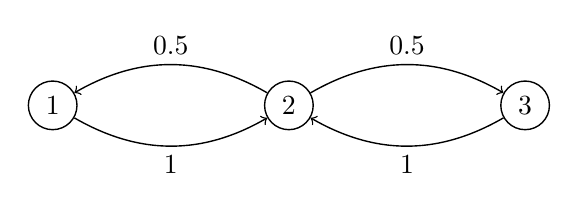
\begin{tikzpicture}[-> , line width=0.5 pt ,node distance =2 cm]
    % \tikzstyle{every node}=[font=\large]
    
    \node[circle, draw] (1) at (0,0) {1};
    \node[circle, draw] (2) at (3,0) {2};
    \node[circle, draw] (3) at (6,0) {3};

    \path (1) edge [bend right] node [below] {$1$} (2);
    \path (2) edge [bend right] node [above] {$0.5$} (1);
    \path (2) edge [bend left] node [above] {$0.5$} (3);
    \path (3) edge [bend left] node [below] {$1$} (2);
    
\end{tikzpicture}
\caption{Ví dụ chuỗi Markov} 
\label{fig:grapheg}
\end{figure}

\noindent Dựa vào đồ thị ta có ma trận chuyển tiếp:
$$
\mathbf{P} = \begin{bmatrix}
    0 & 1 & 0 \\
    0.5 & 0 & 0.5 \\
    0 & 1 & 0
\end{bmatrix}
$$

\noindent Ta có thể thấy nếu luỹ thừa ma trận $\mathbf{P}$ với mũ chẵn thì ta không thể đi từ trạng thái 1 sang trạng thái 2 và không thể đi từ trạng 1 sang trạng thái 3 nếu mũ chẵn. Do đó $\mathbf{P}^n$ luôn tồn tại giá trị $0$ với mọi $n \geq 1$. Vậy chuỗi trên không là một chuỗi chính tắc.
\end{egvn}

\begin{theovn}
    % nếu chuỗi markov là một chuỗi chính tắc và ma trận chuyển tiếp $\mathbf{p}$ chéo hoá được thì tồn tại phân phối bất động. đồng thời phân phối bất động đó chính là chuyển vị của vector riêng tương ứng trị riêng bằng 1 của ma trận $p^t$.
    Nếu chuỗi markov là một chuỗi chính tắc và ma trận chuyển tiếp $\mathbf{P}$ chéo hoá được thì tồn tại phân phối bất động $\pi$. Đặt $e$ là vector riêng ứng với trị riêng bằng 1 của ma trận $\mathbf{P}^T$, khi đó $\pi = e^T$.
\end{theovn}

% % \begin{itemize}
%     % \item Từ phần 2.2, ta đã biết được vector hàng thể hiện trạng thái tại thời điểm $k+1$ với ma trận chuyển tiếp $\mathbf{P}$ được xác định như sau: 
%     % \begin{align}
%     % \pi_{k+1} = \pi_0 \mathbf{P}^k
%     % \end{align}

%     % \item Vậy, điều gì sẽ xảy ra với $k$ tiến dần về dương vô cùng? Liệu rằng vecto trạng thấi tại lúc đó có ``hội tụ'' về một trạng thái ổn định nào đó hay không? Trong đa số trường hợp, câu trả lời là có. Chúng ta hãy xét thử ví dụ dưới đây:

% \noindent Chúng ta có thể giải thích tại sao các phân phối thuộc chuỗi Markov lại có ``hội tụ'' dưới góc nhìn của ma trận. Phương pháp này không thể dùng để chứng minh cho tất cả ma trận Markov, song có thể áp dụng cho đa số các trường hợp. 
    
\begin{proofvn}
    Vì chúng ta vẫn thường thao tác với không gian cột, nên bài chứng minh sẽ xét với ma trận chuyển vị từ hàng thành cột để dễ dàng hình dung hơn.
    \begin{itemize}
        \item Xét ma trận Markov $\mathbf{P}$ chéo hoá được thành $\mathbf{P} = U D U^{-1}$, ta có $\mathbf{P}^T$ cũng chéo hoá được, chứng minh như sau: 
        \begin{align}
            \mathbf{P}^T = (U D U^{-1})^T = (U^{-1})^T D^T U^T = (U^{T})^{-1} D^T U^T
        \end{align}

        \item Đặt $(U^{-1})^T = X$, đồng thời lại có $D^T = D$, từ đó ta được:
        \begin{align}
            \mathbf{P}^T = (U^{-1})^T D^T U^T = X D X^{-1}
        \end{align}

        \item Suy ra $\mathbf{P}^T$ chéo hoá được. Xét ma trận $\mathbf{P}^T$, $X$ là ma trận có các cột là các vector riêng, cột đầu tiên là vector riêng ứng với $\lambda_1 = 1$ , ta được:
        \begin{align}
            \mathbf{P}^T = X D X^{-1}
        \end{align}
        \item Với $\textbf{x}_i$ là các cột của $X, \lambda_i$ là các trị riêng tương ứng với $\textbf{x}_i$, ta được
        \begin{align}
            X = \begin{bmatrix}
            \textbf{x}_1& \textbf{x}_2 & \dots& \textbf{x}_n
            \end{bmatrix}, D = \begin{bmatrix}
            \lambda_1&0& \dotsb &0\\
            0&\lambda_2& \dotsb &0\\
            \vdots & \vdots & \ddots & \vdots\\
            0&0&\dotsb & \lambda_n
            \end{bmatrix}
        \end{align}

        \item Lúc này, $\textbf{x}_i$ là các cột của $X$, phân phối ban đầu $\pi_0$ sẽ được biểu diễn thành tổ hợp tuyến tính của $x_i$ như sau (vì $P^T$ chéo hoá được nên ta sẽ có các vector $x_i$ là cớ sở của không gian $R^{n\text{x}n}$):
        \begin{align}
            \pi_0^T &= c_1 \textbf{x}_1 + c_2 \textbf{x}_2 + ... + c_n \textbf{x}_n \\
            \pi_0^T &= 
            \begin{bmatrix}
                \textbf{x}_1 & ... & \textbf{x}_n 
            \end{bmatrix} 
            \begin{bmatrix}
                c_1 \\
                \vdots \\
                c_n
            \end{bmatrix}\\
            \textbf{c} &= X^{-1} \pi_0^T
        \end{align}

        \item Vector trạng thái sau thời gian $k+1$:
        \begin{align}
            \pi_{k+1} &= \pi_0 \mathbf{P}^k \\
            \Leftrightarrow \hspace{10pt} \pi_{k+1}^T &= (\mathbf{P}^T)^k \pi_0^{T} \\
            \Leftrightarrow \hspace{10pt} \pi_{k+1}^T &= X D^k X^{-1} \pi_0^{T} \\
            \Leftrightarrow \hspace{10pt} \pi_{k+1}^T &= X D^k \textbf{c}
        \end{align}

        \item Ta có:
        \begin{align}
            X D^k =  \begin{bmatrix}
            \textbf{x}_1& \textbf{x}_2 & \dots& \textbf{x}_n
            \end{bmatrix} 
            \begin{bmatrix}
            \lambda_1^k&0& \dotsb &0\\
            0&\lambda_2^k& \dotsb &0\\
            \vdots & \vdots & \ddots & \vdots\\
            0&0&\dotsb & \lambda_n^k
            \end{bmatrix}
        \end{align}
        \item Sử dụng phương pháp nhân hai ma trận (ma trận này nhân với từng cột ma trận kia), ta được:
        \begin{align}
            X D^k =  
            \begin{bmatrix}
            \lambda_1^k\textbf{x}_1& \lambda_2^k\textbf{x}_2 & \dots&\lambda_n^k\textbf{x}_n
            \end{bmatrix} 
        \end{align}

        \item Cùng với quy ước $\lambda_1 = 1$, ta suy ra:
        \begin{align}
            \pi_{k+1}^T &= X D^k C = \begin{bmatrix}
            \lambda_1^k\textbf{x}_1& \lambda_2^k\textbf{x}_2 & \dots&\lambda_n^k\textbf{x}_n
            \end{bmatrix} \begin{bmatrix}
                c_1 \\
                \vdots \\
                c_n
            \end{bmatrix}\\
            &= c_1\textbf{x}_1 + c_2 \lambda_2^k \textbf{x}_2 + ... + c_n \lambda_n^k \textbf{x}_n
        \end{align}

        \item Như đã chứng minh ở mục 2.3, các trị riêng khác 1 và -1 đều có trị tuyệt đối nhỏ hơn 1, chính vì thế khi $k$ càng tăng đến số vô cùng lớn, thì $\pi_{k+1}^T$ sẽ càng tiến gần về $c_1\textbf{x}_1$. Và đây chính là lí do cho sự ``hội tụ'' của các phân phối.

        \item Vậy mới một ma trận Markov chéo hoá được, các phân phối sẽ hội tụ dần về phân phối bất động với phân phối bất động chính là vector riêng tương ứng với trị riêng bằng 1.
    \end{itemize}
\end{proofvn}
% % \end{itemize}

\begin{itemize}
    \item Ở bài chứng minh trên, để tìm được phân phối bất động của 1 ma trận Markov cần phải tính các tham số $c_i$. Tuy nhiên, chúng ta có thể đơn giản hoá nó. Đầu tiên, tìm vector riêng ứng với trị riêng là 1 bằng cách giải phương trình tìm \textbf{x} thoả:
    \begin{align}
        (\mathbf{P}^T - I)\textbf{x} = 0
    \end{align}

    \item Tiếp theo đó, tìm tham số $c$ thoả $c \textbf{x}$ có tổng các phần tử bằng 1 vì $c\textbf{x}^T$ là 1 phân phối. Vậy, ta được phân phối bất động là $c \textbf{x}^T$.
    
    \begin{egvn}
        Thực hành với bài toán thứ hai ở mục 2.3: 
        \begin{itemize}
        \item Ta có ma trận Markov $\mathbf{P}$:
        \begin{align}
            \begin{bmatrix}
                0.80 & 0.20 \\
                0.10 & 0.90 
            \end{bmatrix}
        \end{align}
    
        \item Và phân phối ban đầu $\pi_0$:
                $$\begin{bmatrix}
                        0.6 & 0.4  
                \end{bmatrix}$$
    
        \item Giải phương trình: 
        \begin{align}
            (\mathbf{P}^T - I)\textbf{x} = 0
        \end{align}
    
        \item Ta được nghiệm:
        \begin{align}
            \textbf{x}^T = \begin{bmatrix}
                1 & 2
            \end{bmatrix}
        \end{align}
    
        \item Từ đó dễ dàng tìm được $c = \dfrac{1}{3}$. Suy ra phân phối bất động là $$
        \pi =
        \begin{bmatrix}
            \dfrac{1}{3} & \dfrac{2}{3}
        \end{bmatrix} $$.
    
        \item Từ đó, chúng ta có thể dự đoán rằng, trong tương lai nếu không biến cố nào xảy ra gây ảnh hưởng đến ma trận chuyển tiếp, thì điện thoại IOS sẽ chiếm $\dfrac{2}{3}$ thị phần, còn Android chiếm $\dfrac{1}{3}$ thị phần. 
        
        \end{itemize}
    \end{egvn}
\end{itemize}